% Options for packages loaded elsewhere
\PassOptionsToPackage{unicode}{hyperref}
\PassOptionsToPackage{hyphens}{url}
%
\documentclass[
]{book}
\usepackage{amsmath,amssymb}
\usepackage{lmodern}
\usepackage{iftex}
\ifPDFTeX
  \usepackage[T1]{fontenc}
  \usepackage[utf8]{inputenc}
  \usepackage{textcomp} % provide euro and other symbols
\else % if luatex or xetex
  \usepackage{unicode-math}
  \defaultfontfeatures{Scale=MatchLowercase}
  \defaultfontfeatures[\rmfamily]{Ligatures=TeX,Scale=1}
\fi
% Use upquote if available, for straight quotes in verbatim environments
\IfFileExists{upquote.sty}{\usepackage{upquote}}{}
\IfFileExists{microtype.sty}{% use microtype if available
  \usepackage[]{microtype}
  \UseMicrotypeSet[protrusion]{basicmath} % disable protrusion for tt fonts
}{}
\makeatletter
\@ifundefined{KOMAClassName}{% if non-KOMA class
  \IfFileExists{parskip.sty}{%
    \usepackage{parskip}
  }{% else
    \setlength{\parindent}{0pt}
    \setlength{\parskip}{6pt plus 2pt minus 1pt}}
}{% if KOMA class
  \KOMAoptions{parskip=half}}
\makeatother
\usepackage{xcolor}
\usepackage{color}
\usepackage{fancyvrb}
\newcommand{\VerbBar}{|}
\newcommand{\VERB}{\Verb[commandchars=\\\{\}]}
\DefineVerbatimEnvironment{Highlighting}{Verbatim}{commandchars=\\\{\}}
% Add ',fontsize=\small' for more characters per line
\usepackage{framed}
\definecolor{shadecolor}{RGB}{248,248,248}
\newenvironment{Shaded}{\begin{snugshade}}{\end{snugshade}}
\newcommand{\AlertTok}[1]{\textcolor[rgb]{0.94,0.16,0.16}{#1}}
\newcommand{\AnnotationTok}[1]{\textcolor[rgb]{0.56,0.35,0.01}{\textbf{\textit{#1}}}}
\newcommand{\AttributeTok}[1]{\textcolor[rgb]{0.77,0.63,0.00}{#1}}
\newcommand{\BaseNTok}[1]{\textcolor[rgb]{0.00,0.00,0.81}{#1}}
\newcommand{\BuiltInTok}[1]{#1}
\newcommand{\CharTok}[1]{\textcolor[rgb]{0.31,0.60,0.02}{#1}}
\newcommand{\CommentTok}[1]{\textcolor[rgb]{0.56,0.35,0.01}{\textit{#1}}}
\newcommand{\CommentVarTok}[1]{\textcolor[rgb]{0.56,0.35,0.01}{\textbf{\textit{#1}}}}
\newcommand{\ConstantTok}[1]{\textcolor[rgb]{0.00,0.00,0.00}{#1}}
\newcommand{\ControlFlowTok}[1]{\textcolor[rgb]{0.13,0.29,0.53}{\textbf{#1}}}
\newcommand{\DataTypeTok}[1]{\textcolor[rgb]{0.13,0.29,0.53}{#1}}
\newcommand{\DecValTok}[1]{\textcolor[rgb]{0.00,0.00,0.81}{#1}}
\newcommand{\DocumentationTok}[1]{\textcolor[rgb]{0.56,0.35,0.01}{\textbf{\textit{#1}}}}
\newcommand{\ErrorTok}[1]{\textcolor[rgb]{0.64,0.00,0.00}{\textbf{#1}}}
\newcommand{\ExtensionTok}[1]{#1}
\newcommand{\FloatTok}[1]{\textcolor[rgb]{0.00,0.00,0.81}{#1}}
\newcommand{\FunctionTok}[1]{\textcolor[rgb]{0.00,0.00,0.00}{#1}}
\newcommand{\ImportTok}[1]{#1}
\newcommand{\InformationTok}[1]{\textcolor[rgb]{0.56,0.35,0.01}{\textbf{\textit{#1}}}}
\newcommand{\KeywordTok}[1]{\textcolor[rgb]{0.13,0.29,0.53}{\textbf{#1}}}
\newcommand{\NormalTok}[1]{#1}
\newcommand{\OperatorTok}[1]{\textcolor[rgb]{0.81,0.36,0.00}{\textbf{#1}}}
\newcommand{\OtherTok}[1]{\textcolor[rgb]{0.56,0.35,0.01}{#1}}
\newcommand{\PreprocessorTok}[1]{\textcolor[rgb]{0.56,0.35,0.01}{\textit{#1}}}
\newcommand{\RegionMarkerTok}[1]{#1}
\newcommand{\SpecialCharTok}[1]{\textcolor[rgb]{0.00,0.00,0.00}{#1}}
\newcommand{\SpecialStringTok}[1]{\textcolor[rgb]{0.31,0.60,0.02}{#1}}
\newcommand{\StringTok}[1]{\textcolor[rgb]{0.31,0.60,0.02}{#1}}
\newcommand{\VariableTok}[1]{\textcolor[rgb]{0.00,0.00,0.00}{#1}}
\newcommand{\VerbatimStringTok}[1]{\textcolor[rgb]{0.31,0.60,0.02}{#1}}
\newcommand{\WarningTok}[1]{\textcolor[rgb]{0.56,0.35,0.01}{\textbf{\textit{#1}}}}
\usepackage{longtable,booktabs,array}
\usepackage{calc} % for calculating minipage widths
% Correct order of tables after \paragraph or \subparagraph
\usepackage{etoolbox}
\makeatletter
\patchcmd\longtable{\par}{\if@noskipsec\mbox{}\fi\par}{}{}
\makeatother
% Allow footnotes in longtable head/foot
\IfFileExists{footnotehyper.sty}{\usepackage{footnotehyper}}{\usepackage{footnote}}
\makesavenoteenv{longtable}
\usepackage{graphicx}
\makeatletter
\def\maxwidth{\ifdim\Gin@nat@width>\linewidth\linewidth\else\Gin@nat@width\fi}
\def\maxheight{\ifdim\Gin@nat@height>\textheight\textheight\else\Gin@nat@height\fi}
\makeatother
% Scale images if necessary, so that they will not overflow the page
% margins by default, and it is still possible to overwrite the defaults
% using explicit options in \includegraphics[width, height, ...]{}
\setkeys{Gin}{width=\maxwidth,height=\maxheight,keepaspectratio}
% Set default figure placement to htbp
\makeatletter
\def\fps@figure{htbp}
\makeatother
\setlength{\emergencystretch}{3em} % prevent overfull lines
\providecommand{\tightlist}{%
  \setlength{\itemsep}{0pt}\setlength{\parskip}{0pt}}
\setcounter{secnumdepth}{5}
\usepackage{booktabs}
%\usepackage{zi4}
\usepackage[hangul]{kotex}
\usepackage{makeidx}
\usepackage{imakeidx}
\makeindex[columns=2]
\usepackage{fixltx2e}
\usepackage{fvextra} \DefineVerbatimEnvironment{Highlighting}{Verbatim}{breaklines,commandchars=\\\{\}}
\ifLuaTeX
  \usepackage{selnolig}  % disable illegal ligatures
\fi
\usepackage[]{natbib}
\bibliographystyle{plainnat}
\IfFileExists{bookmark.sty}{\usepackage{bookmark}}{\usepackage{hyperref}}
\IfFileExists{xurl.sty}{\usepackage{xurl}}{} % add URL line breaks if available
\urlstyle{same} % disable monospaced font for URLs
\hypersetup{
  pdftitle={R로 알아가는 시계열분석},
  pdfauthor={박동련},
  hidelinks,
  pdfcreator={LaTeX via pandoc}}

\title{R로 알아가는 시계열분석}
\author{박동련}
\date{}

\begin{document}
\maketitle

{
\setcounter{tocdepth}{1}
\tableofcontents
}
\hypertarget{uxba38uxb9acuxb9d0}{%
\chapter*{머리말}\label{uxba38uxb9acuxb9d0}}
\addcontentsline{toc}{chapter}{머리말}

시간의 흐름에 따라 관측되는 시계열자료는 경영\(\cdot\)경제 분야 뿐 아니라 이제는 다른 많은 분야에서도 흔히 접할 수 있는 형태의 자료이다. 시계열자료의 가장 큰 특징은 자료들 사이에 강한 상관관계가 존재할 수 있다는 것인데, 이런 특징으로 인하여 선형회귀모형과 같이 자료의 독립성을 가정으로 하고 있는 모형으로는 시계열자료의 분석에 한계가 있다.

이 책은 교우사에서 출판한 ``R로 알아가는 시계열분석''에서 사용된 R code와 더불어 실습 예제만을 추려서 HTML 버전으로 다시 작성한 것으로, 독자들의 R 실습에 조그만한 도움이 되고자 작성하였다.

이 책애서 가장 많이 사용되는 예측 기법인 ETS 모형과 ARIMA 모형, 그리고 ARMA 오차 회귀모형을 다루고 있으며, 특히 패키지 \texttt{forecast}의 다양한 함수의 활용 방법을 소개하고 있다. 패키지 \texttt{forecast}{[}\url{https://pkg.robjhyndman.com/forecast/}{]}는 시계열분석에서 가장 많이 사용되는 R 패키지 중 하나이다.

이 책은 패키지 \texttt{bookdown}{[}\url{https://bookdown.org/}{]}을 사용하여 Rstudio에서 작성되었으며, R의 기초적인 사용법 및 패키지 \texttt{tidyverse}{[}\url{https://www.tidyverse.org/}{]}에 대한 소개 없이 사용하고 있다. 또한 R code에는 프롬프트(\texttt{\textgreater{}} 또는 \texttt{+})를 제거하였고, console 창에 출력되는 실행 결과물은 \texttt{\#\#}으로 시작되도록 하였다.

제공된 R code는 마우스를 code 블록의 오른쪽 상단 구석에 놓으면 블록 전체를 복사할 수 있는 기호가 다음과 같이 나타난다.

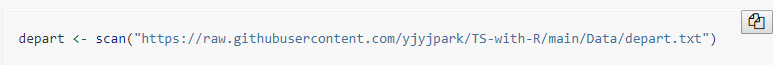
\includegraphics{Figures/code-block.png}

이 책을 작성할 때의 R 세션 정보는 다음과 같다.

\begin{Shaded}
\begin{Highlighting}[]
\FunctionTok{sessionInfo}\NormalTok{()}
\end{Highlighting}
\end{Shaded}

\begin{verbatim}
## R version 4.2.1 (2022-06-23 ucrt)
## Platform: x86_64-w64-mingw32/x64 (64-bit)
## Running under: Windows 10 x64 (build 22621)
## 
## Matrix products: default
## 
## locale:
## [1] LC_COLLATE=Korean_Korea.utf8 
## [2] LC_CTYPE=Korean_Korea.utf8   
## [3] LC_MONETARY=Korean_Korea.utf8
## [4] LC_NUMERIC=C                 
## [5] LC_TIME=Korean_Korea.utf8    
## 
## attached base packages:
## [1] stats     graphics  grDevices utils     datasets 
## [6] methods   base     
## 
## other attached packages:
##  [1] expsmooth_2.3   fma_2.4         forecast_8.18  
##  [4] fpp2_2.4        forcats_0.5.2   stringr_1.4.1  
##  [7] dplyr_1.0.10    purrr_0.3.5     readr_2.1.3    
## [10] tidyr_1.2.1     tibble_3.1.8    ggplot2_3.3.6  
## [13] tidyverse_1.3.2
## 
## loaded via a namespace (and not attached):
##  [1] tseries_0.10-52     httr_1.4.4         
##  [3] jsonlite_1.8.3      modelr_0.1.9       
##  [5] assertthat_0.2.1    TTR_0.24.3         
##  [7] googlesheets4_1.0.1 cellranger_1.1.0   
##  [9] yaml_2.3.6          pillar_1.8.1       
## [11] backports_1.4.1     lattice_0.20-45    
## [13] glue_1.6.2          quadprog_1.5-8     
## [15] digest_0.6.30       rvest_1.0.3        
## [17] colorspace_2.0-3    htmltools_0.5.3    
## [19] timeDate_4021.106   pkgconfig_2.0.3    
## [21] broom_1.0.1         haven_2.5.1        
## [23] bookdown_0.29       scales_1.2.1       
## [25] tzdb_0.3.0          googledrive_2.0.0  
## [27] generics_0.1.3      ellipsis_0.3.2     
## [29] withr_2.5.0         urca_1.3-3         
## [31] nnet_7.3-17         cli_3.4.1          
## [33] quantmod_0.4.20     magrittr_2.0.3     
## [35] crayon_1.5.2        readxl_1.4.1       
## [37] evaluate_0.17       fs_1.5.2           
## [39] fansi_1.0.3         nlme_3.1-157       
## [41] xts_0.12.2          xml2_1.3.3         
## [43] tools_4.2.1         hms_1.1.2          
## [45] gargle_1.2.1        lifecycle_1.0.3    
## [47] munsell_0.5.0       reprex_2.0.2       
## [49] compiler_4.2.1      rlang_1.0.6        
## [51] grid_4.2.1          rstudioapi_0.14    
## [53] rmarkdown_2.17      gtable_0.3.1       
## [55] fracdiff_1.5-1      curl_4.3.3         
## [57] DBI_1.1.3           R6_2.5.1           
## [59] zoo_1.8-11          lubridate_1.8.0    
## [61] knitr_1.40          fastmap_1.1.0      
## [63] utf8_1.2.2          stringi_1.7.8      
## [65] parallel_4.2.1      Rcpp_1.0.9         
## [67] vctrs_0.5.0         dbplyr_2.2.1       
## [69] tidyselect_1.2.0    xfun_0.34          
## [71] lmtest_0.9-40
\end{verbatim}

\hypertarget{chapter-ts-plot}{%
\chapter{시계열 그래프}\label{chapter-ts-plot}}

Placeholder

\hypertarget{uxc2dcuxacc4uxc5f4uxc790uxb8cc}{%
\section{시계열자료}\label{uxc2dcuxacc4uxc5f4uxc790uxb8cc}}

\hypertarget{uxc2dcuxacc4uxc5f4-uxadf8uxb798uxd504-uxc791uxc131}{%
\section{시계열 그래프 작성}\label{uxc2dcuxacc4uxc5f4-uxadf8uxb798uxd504-uxc791uxc131}}

\hypertarget{ts-uxac1duxccb4-uxc0dduxc131}{%
\subsection{\texorpdfstring{\texttt{ts} 객체 생성}{ts 객체 생성}}\label{ts-uxac1duxccb4-uxc0dduxc131}}

\hypertarget{section-ts-plot}{%
\subsection{시계열 그래프 작성}\label{section-ts-plot}}

\hypertarget{section-seasonal-plot}{%
\subsection{Seasonal 그래프}\label{section-seasonal-plot}}

  \bibliography{book.bib,packages.bib}

\printindex

\end{document}
